\documentclass{article}
\usepackage{ctex}     % 导入 ctex 宏包
\usepackage{amsmath}  % 提供数学公式排版功能
\usepackage{amssymb}  % 提供额外的数学符号
\usepackage{graphicx} % 插入图片
\usepackage{float}    % 图表位置
\usepackage{geometry} % 控制页面布局
\usepackage{subcaption}
\usepackage{listings}
\usepackage{xcolor}
\usepackage{url}
\geometry{a4paper, margin=1in} % 设置纸张大小和边距
\lstset{
    basicstyle=\ttfamily\footnotesize,
    keywordstyle=\color{blue},
    commentstyle=\color{gray},
    stringstyle=\color{red},
    numbers=left,
    numberstyle=\tiny\color{gray},
    stepnumber=1,
    numbersep=5pt,
    backgroundcolor=\color{white},
    showspaces=false,
    showstringspaces=false,
    showtabs=false,
    frame=single,
    tabsize=2,
    captionpos=b,
    breaklines=true,
    breakatwhitespace=false,
    escapeinside={\%*}{*)}
}

% 设置中文字体为楷体
\setCJKmainfont{KaiTi} % 设置主字体为楷体
\setCJKsansfont{KaiTi} % 设置无衬线字体为楷体
\setCJKmonofont{KaiTi} % 设置等宽字体为楷体

\title{HW1：螺丝图像的单应估计与矫正}
\author{李青雅 523030910004 电院2301}
\date{\today} % 自动插入今天的日期

\begin{document}
\maketitle
\newpage
\tableofcontents % 生成目录
\newpage

\section{方法概述}
本作业的目标是将视角倾斜的图像矫正为与模板一致的俯视图。整体思路可以概括为：在模板图与待处理图中找到同一位置的显著特征点，依据这些对应点计算一套几何映射关系，再利用该映射将整幅图像拉正并对齐到模板坐标系。

第一步为图像读取与灰度化处理。将彩色图像转换为灰度图后，能够保留主要结构信息并减弱颜色差异带来的干扰，使特征更稳定、匹配更可靠。

第二步为特征点与描述子提取。特征点可理解为图中纹理变化明显、具有辨识度的位置；描述子是对这些位置局部图像的数字化刻画，用于跨图像匹配。本文采用 ORB 方法（Oriented FAST and Rotated BRIEF），其核心思想是先用 FAST 算法快速检测角点，再为角点估计主方向，最后用 BRIEF 生成简洁的二进制描述子，从而在保证速度的同时对图像旋转具有一定鲁棒性。

第三步为特征匹配与筛选。通过最近邻匹配寻找最相似的描述子对，并采用比例测试剔除不可靠的匹配关系，以降低误匹配对后续估计的影响。

第四步为单应矩阵估计。单应矩阵刻画了平面场景在两张图之间的几何变换关系，其形式为一个 $3\times3$ 矩阵：
\begin{equation}
H=
\begin{bmatrix}
h_{11} & h_{12} & h_{13} \\
h_{21} & h_{22} & h_{23} \\
h_{31} & h_{32} & h_{33}
\end{bmatrix},
\end{equation}
并满足齐次坐标下的映射关系 $(x',y',1)^\mathsf{T} \sim H(x,y,1)^\mathsf{T}$。为抵御少量错误匹配的干扰，使用 RANSAC 进行鲁棒估计。RANSAC 会反复从匹配点中随机抽取最小样本估计 $H$，再用重投影误差筛选内点，最终选择内点数最多的一组结果。

第五步为透视变换与结果输出。利用估计得到的单应矩阵对整幅图像进行透视变换，使其对齐到模板图的坐标与尺寸，最终得到矫正后的俯视图。

\section{参数设置}
主要参数设置如下：ORB（Oriented FAST and Rotated BRIEF）特征点数量设为 5000，匹配比例阈值为 0.75，RANSAC 重投影阈值为 5.0，最大迭代次数为 5000，置信度为 0.995。在 ORB 匹配内点数低于 10 时，使用 AKAZE 作为补充特征提取器重新估计单应矩阵。AKAZE 的特点是使用非线性尺度空间提取特征，对纹理较弱或尺度变化较大的情况更稳健，因此可作为 ORB 的补充以提升整体稳定性。

以样例图像 raw\_01\_warp1.png 为例，实际计算得到的单应矩阵为：
\begin{equation}
H=
\begin{bmatrix}
0.823187 & -0.220794 & 173.684171 \\
0.123021 & 0.716824 & -475.851563 \\
-0.000008 & -0.000044 & 1.000000
\end{bmatrix}.
\end{equation}

\section{结果与分析}
所有 60 张图像均成功输出到与模板一致的尺寸。绝大部分结果矫正效果良好，raw\_02 与 raw\_03 系列中存在少量轻微倾斜的样本，且仅 raw\_10\_warp6 出现明显失败。根据图像质量与匹配情况，可将处理策略概括为三种情形。第一种是视角变化较小且纹理清晰的样本，ORB 匹配内点较多，直接使用 ORB+RANSAC 得到稳定单应矩阵，矫正后结构纹理与模板对齐明显。第二种是视角变化较大或螺丝遮挡较多的样本，匹配内点数量下降，此时仍采用 RANSAC 进行鲁棒估计，确保主要平面结构得到恢复。第三种是特征稀疏或内点不足的样本，当 ORB 内点数低于阈值时切换至 AKAZE 重新估计单应矩阵，以提升在弱纹理与尺度变化场景下的稳定性并保证输出连续性。

图 \ref{fig:good} 展示了效果较好的样例 raw\_01\_warp1.png，几何结构与模板基本对齐。图 \ref{fig:slight} 为 raw\_02\_warp5.png，结果较原始图像有明显改善，但仍存在一定倾斜，主要表现为边缘线条与模板存在夹角。
\begin{figure}[H]
    \centering
    \begin{subfigure}[t]{0.26\linewidth}
        \centering
        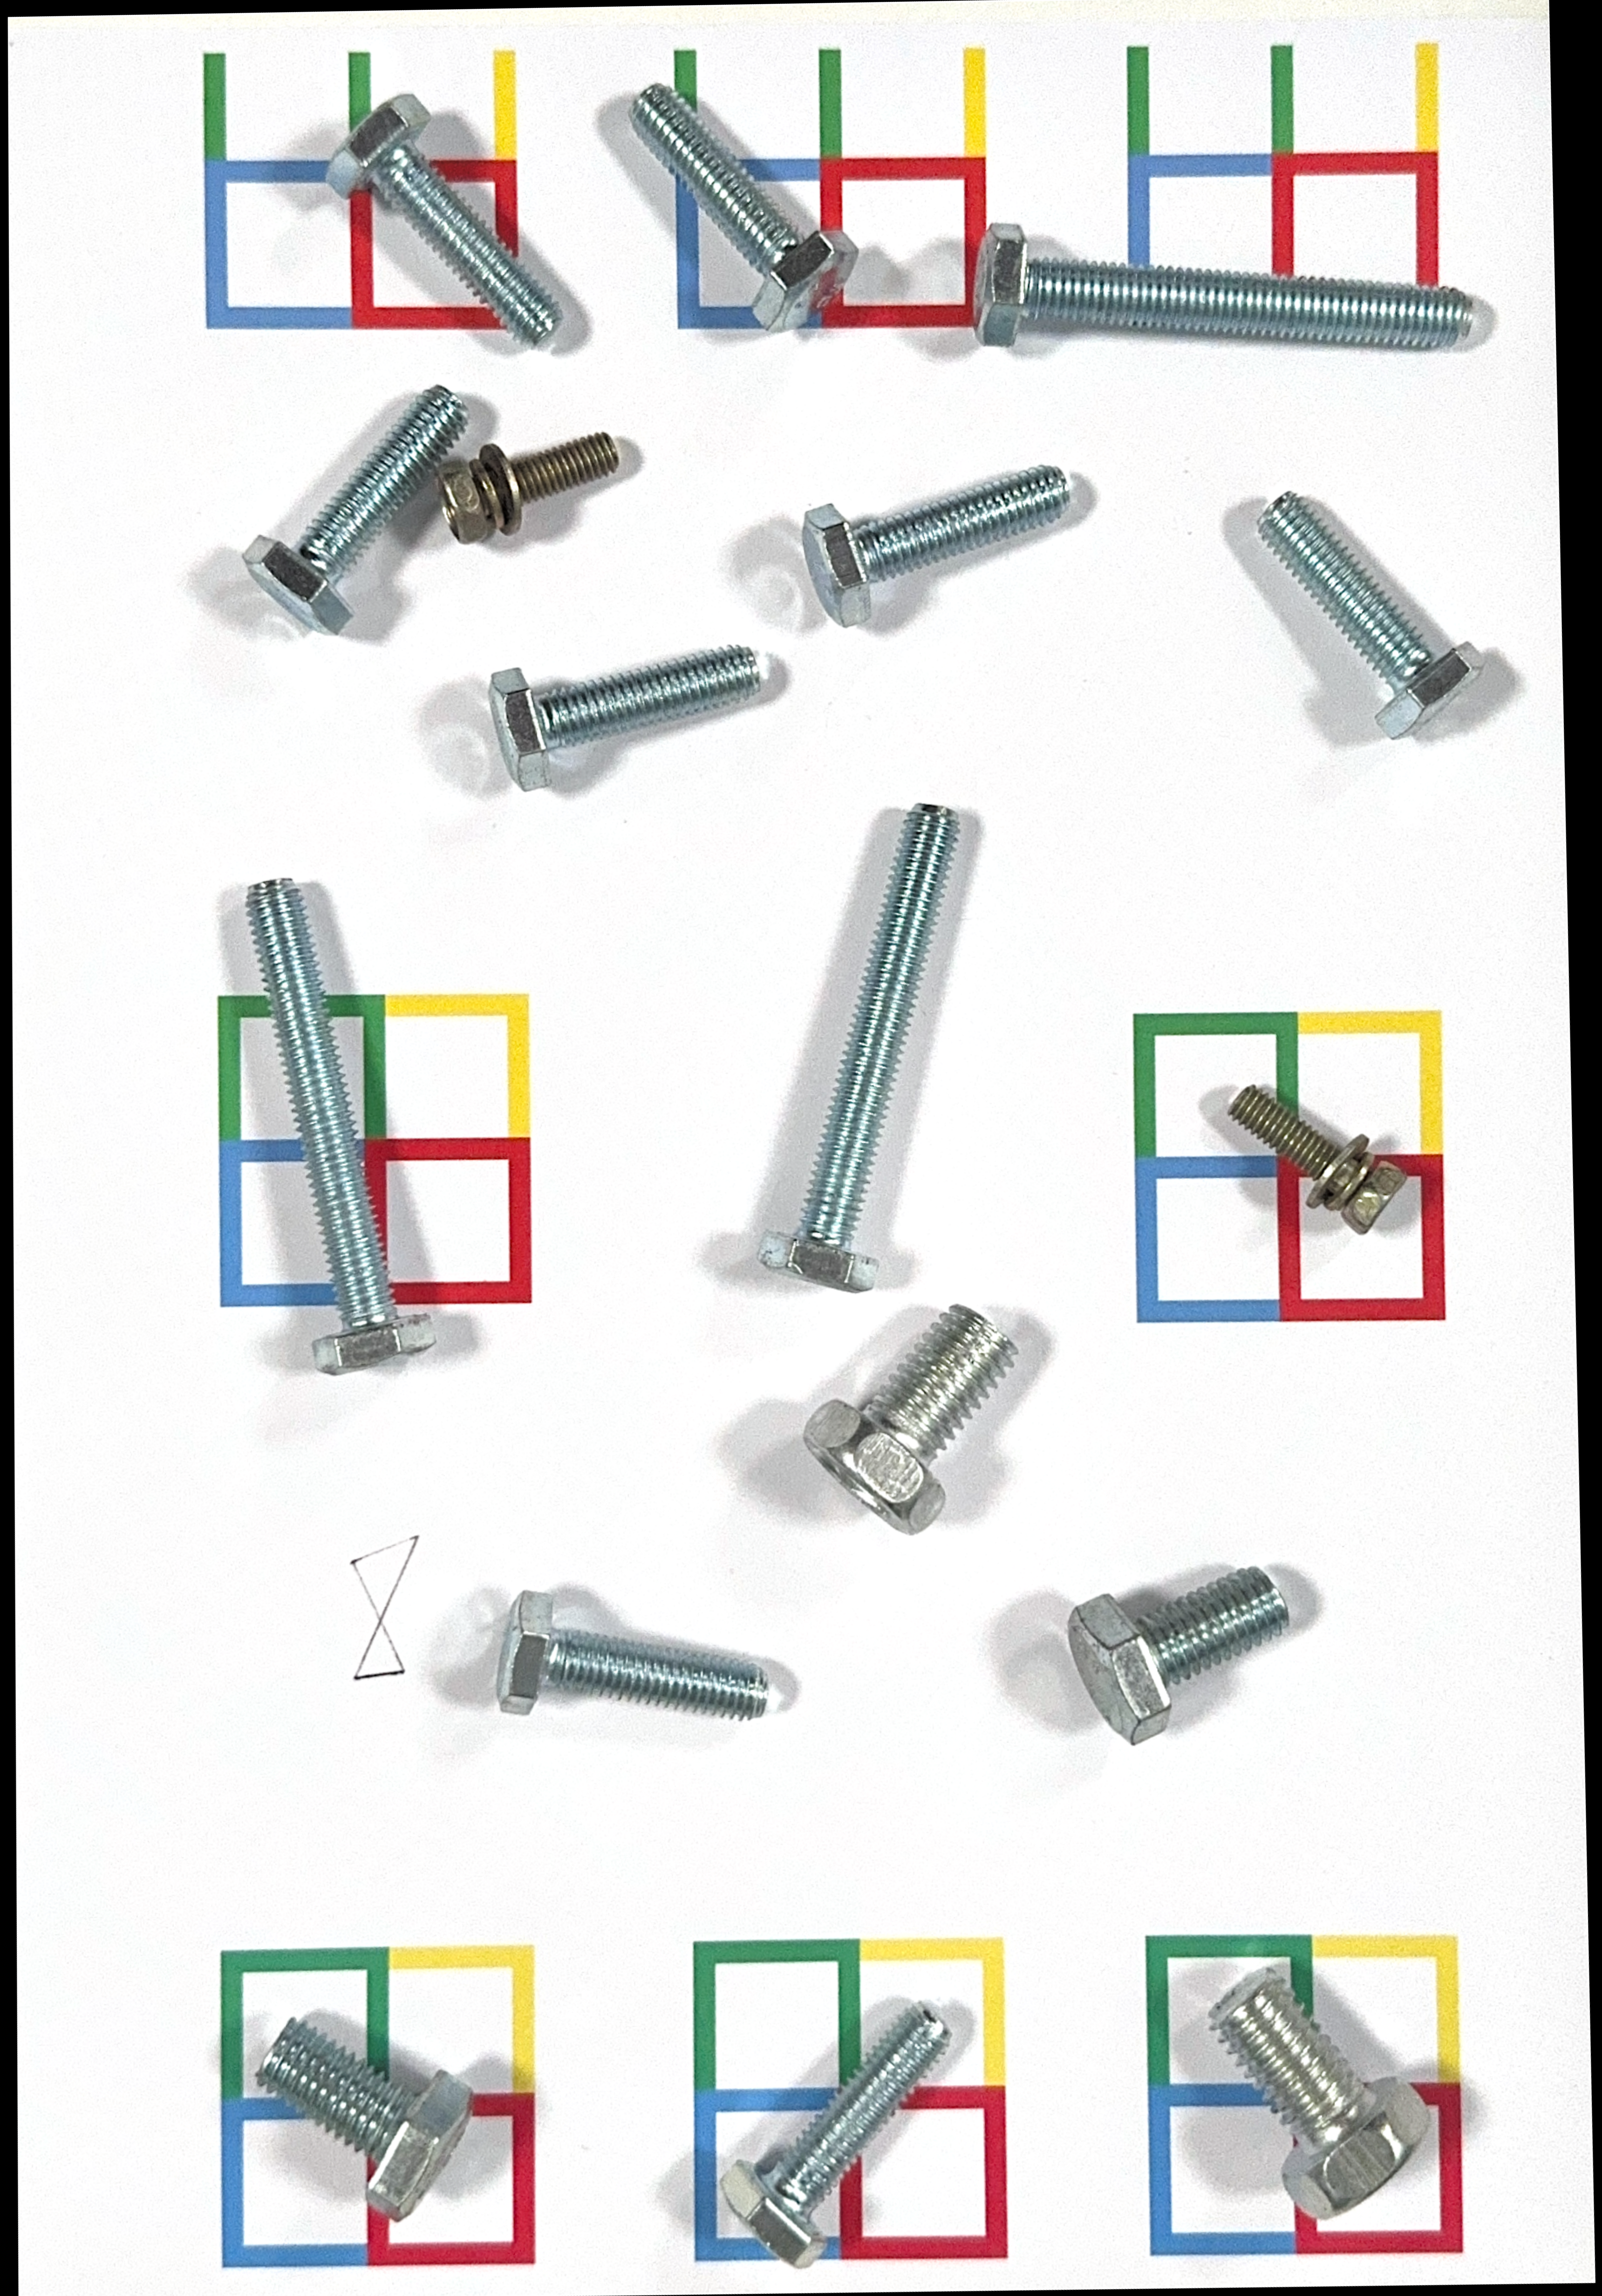
\includegraphics[width=\linewidth]{../523030910004_submission/restored_images/raw_01_warp1.png}
        \caption{矫正效果较好的样例 raw\_01\_warp1}
        \label{fig:good}
    \end{subfigure}
    \hspace{0.01\linewidth}
    \begin{subfigure}[t]{0.26\linewidth}
        \centering
        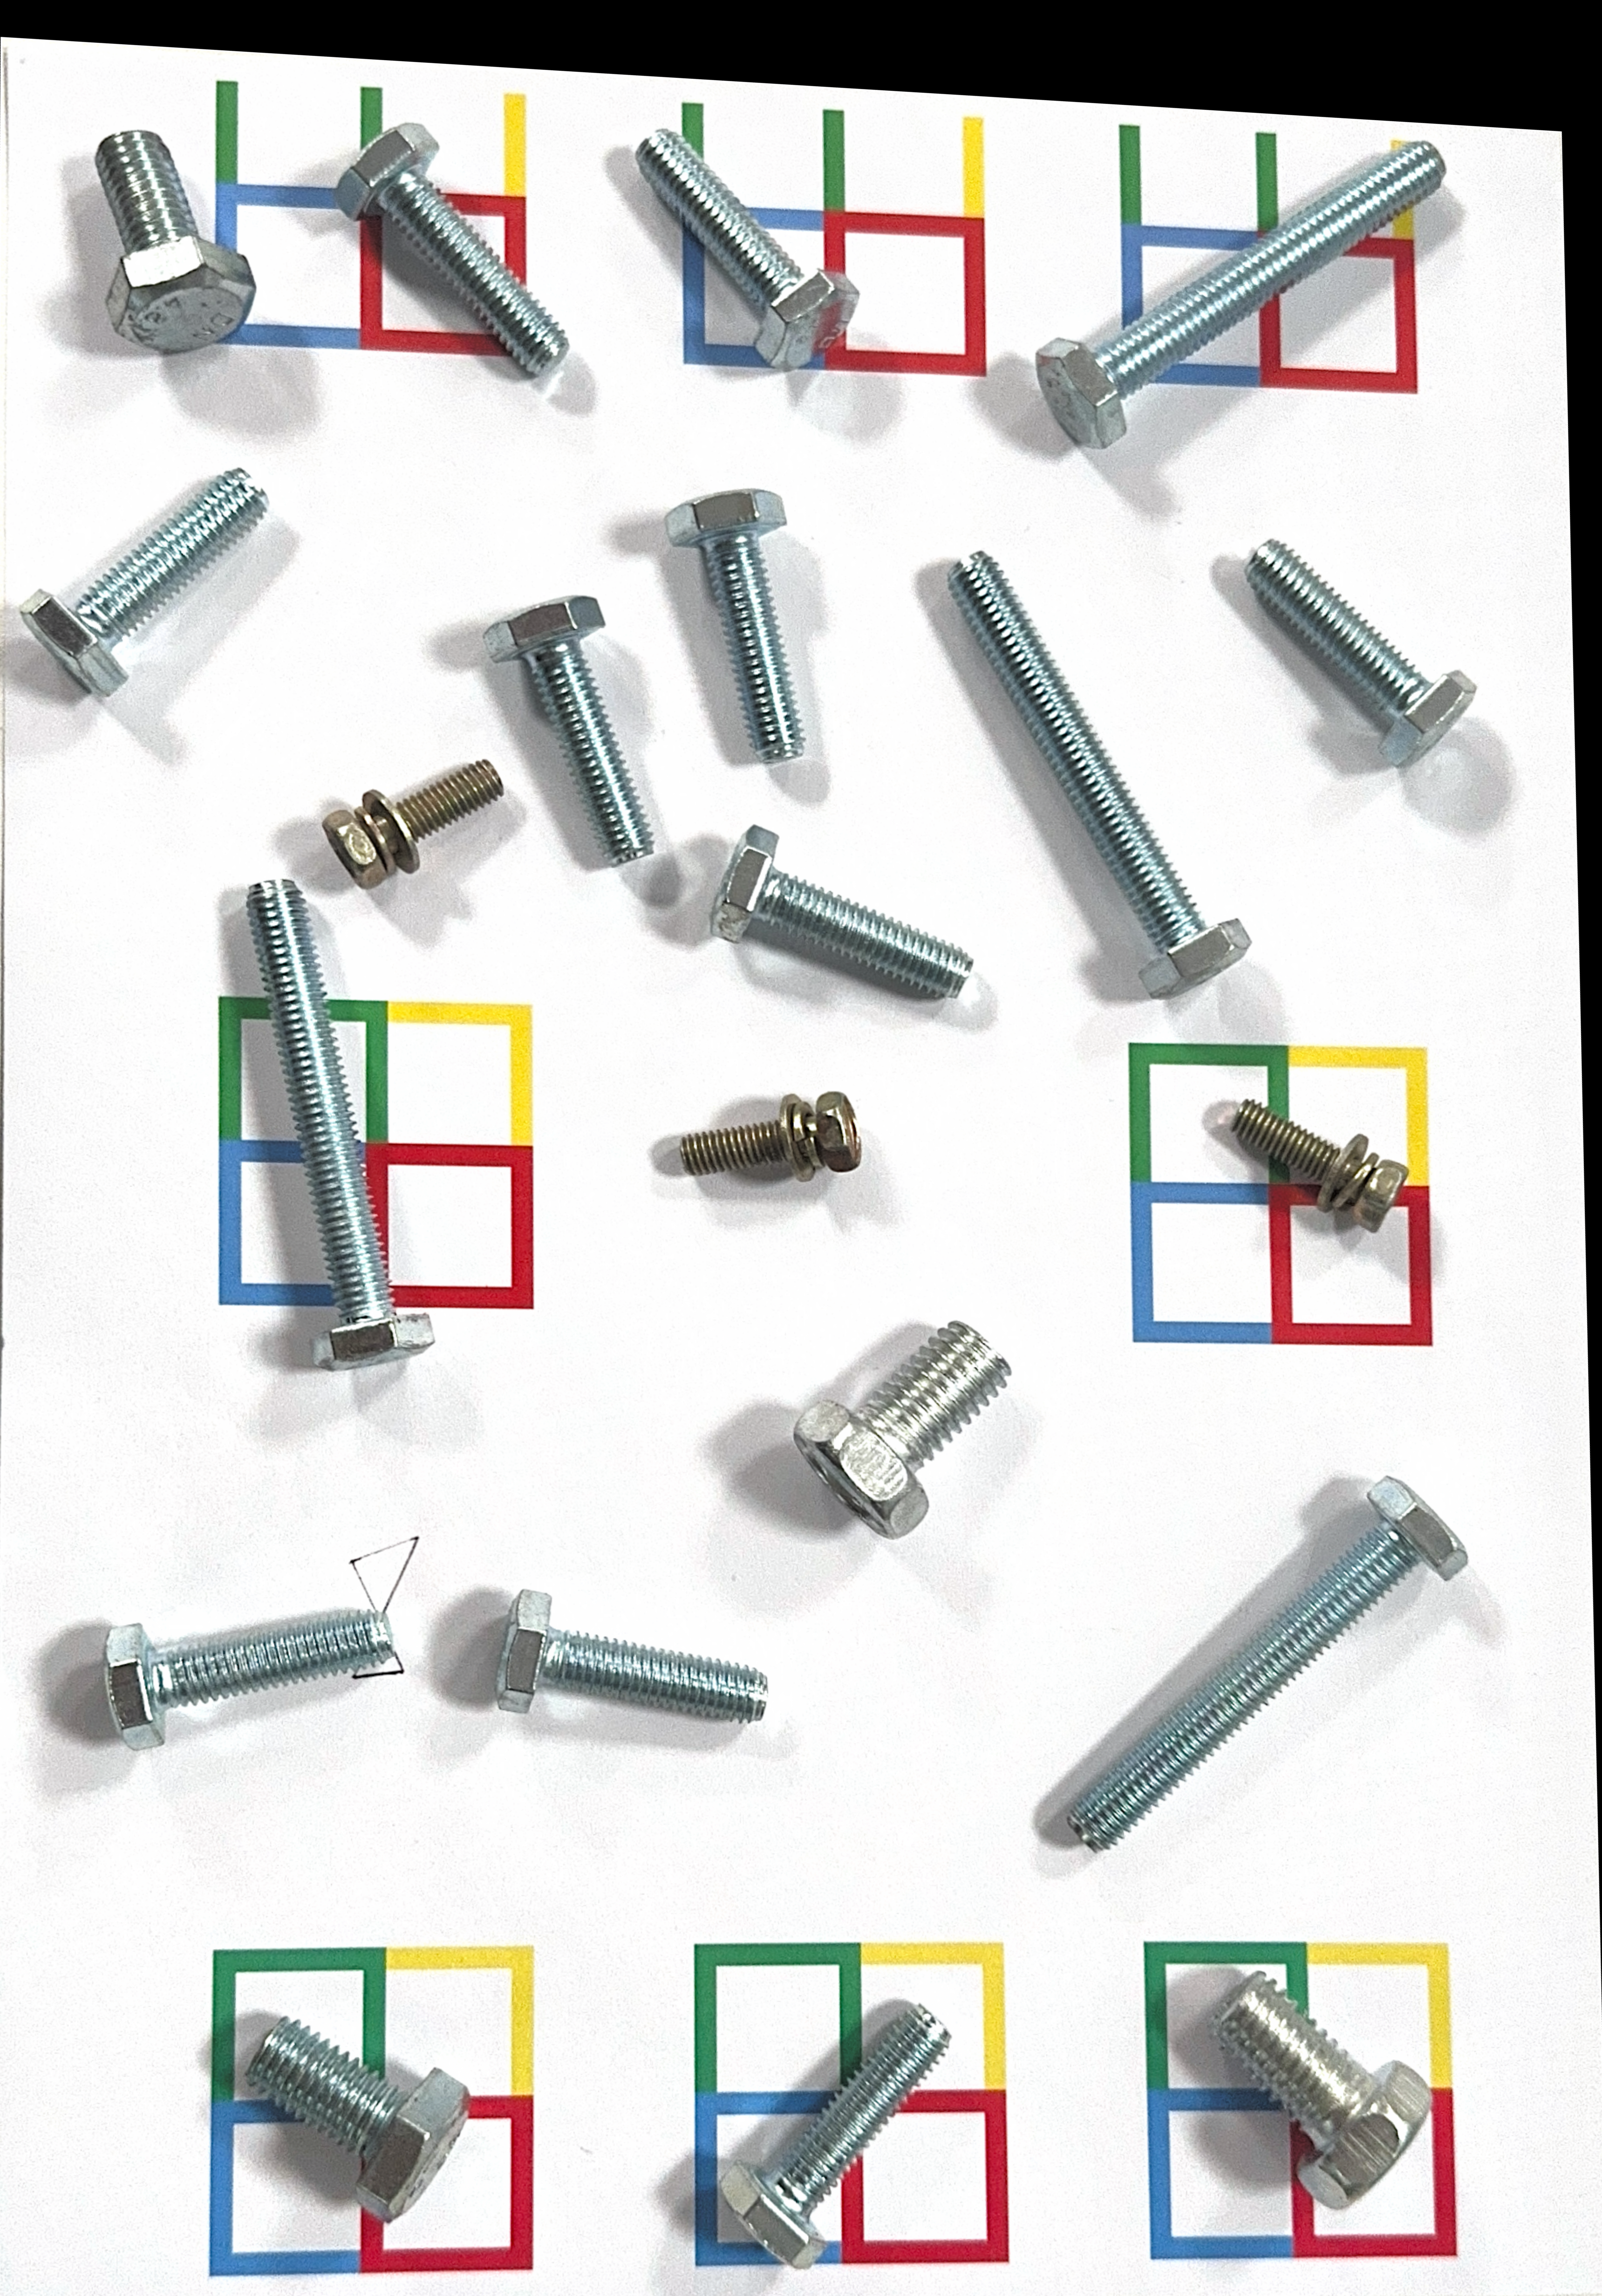
\includegraphics[width=\linewidth]{../523030910004_submission/restored_images/raw_02_warp5.png}
        \caption{矫正有改善但仍略微倾斜的样例 raw\_02\_warp5}
        \label{fig:slight}
    \end{subfigure}
    \caption{结果对比示例}
\end{figure}

\section{失败案例与原因}
彻底失败样例为 raw\_10\_warp6.png，如图 \ref{fig:fail-compare} 所示。该样本失败的主要原因包括：其一，视角变化与透视形变幅度过大，平面在图像中被强烈拉伸与倾斜，使得同一平面的几何约束变得脆弱；其二，可用纹理集中在局部区域，特征点分布不均匀，导致估计的单应矩阵被局部结构主导，无法代表整体平面；其三，螺丝遮挡与背景空白区域共同增加了误匹配概率，RANSAC 在少量外点的影响下仍可能被拉偏，最终产生整体扭曲与拉伸。
\begin{figure}[H]
    \centering
    \begin{subfigure}[t]{0.26\linewidth}
        \centering
        
\includegraphics[width=\linewidth]{../HW1_data/raw_10_warp6.png}
        \caption{原始图像 raw\_10\_warp6}
    \end{subfigure}
    \hspace{0.01\linewidth}
    \begin{subfigure}[t]{0.26\linewidth}
        \centering
        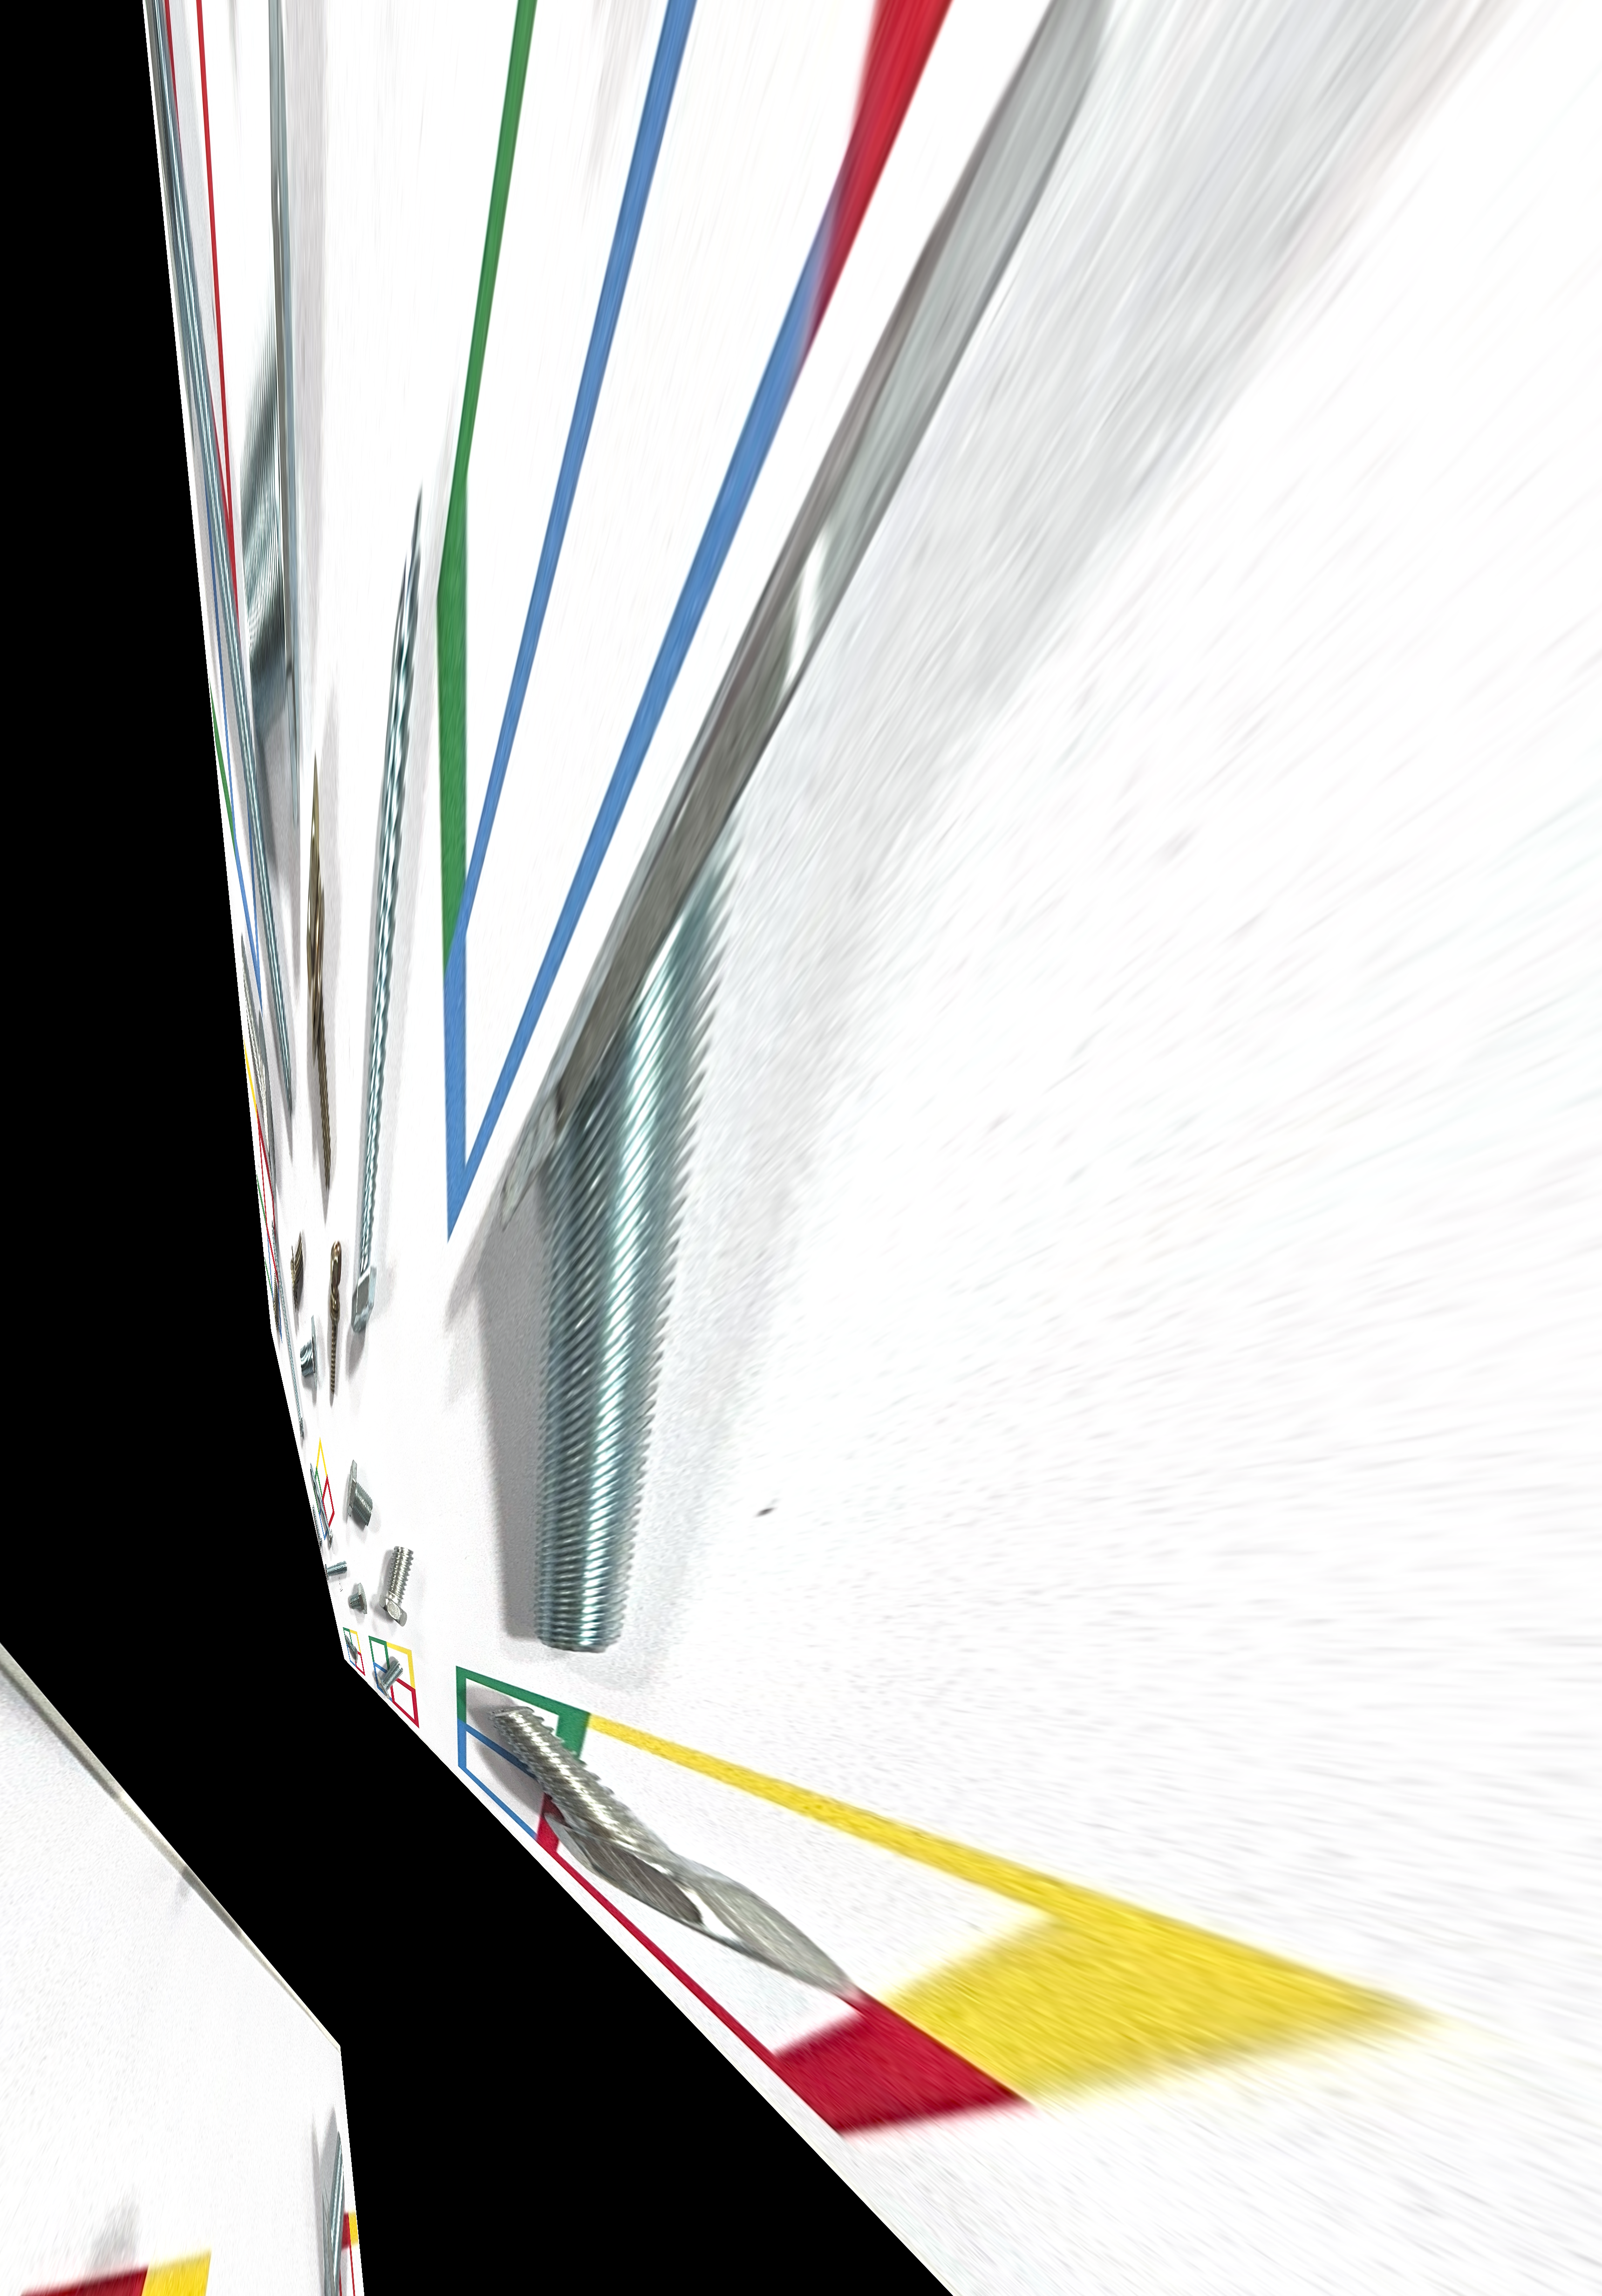
\includegraphics[width=\linewidth]{../523030910004_submission/restored_images/raw_10_warp6.png}
        \caption{矫正结果 raw\_10\_warp6}
    \end{subfigure}
    \caption{失败样例的原始图像与矫正结果对比}
    \label{fig:fail-compare}
\end{figure}

\section{关键改动}
针对 raw\_10\_warp6.png 的失败样例，新增了“单图强化处理”脚本，主要改动如下：增加特征点数量并同时使用 ORB 与 AKAZE 两种检测器进行估计；引入网格均匀采样，限制每个网格内的匹配点数量，使匹配点覆盖全图，减轻局部结构主导的问题；将匹配比例阈值收紧以降低误匹配，并提高 RANSAC 迭代次数以提升鲁棒性。具体参数为：nfeatures=8000，ratio=0.7，grid\_rows=4，grid\_cols=4，max\_per\_cell=30，RANSAC 最大迭代次数 8000，重投影阈值 5.0，置信度 0.995。

图 \ref{fig:refined-compare} 给出原始图、原始脚本矫正结果以及改进脚本的矫正结果并排对比。
\begin{figure}[H]
    \centering
    \begin{subfigure}[t]{0.26\linewidth}
        \centering
        
\includegraphics[width=\linewidth]{../HW1_data/raw_10_warp6.png}
        \caption{原始图像 raw\_10\_warp6}
    \end{subfigure}
    \hspace{0.01\linewidth}
    \begin{subfigure}[t]{0.26\linewidth}
        \centering
        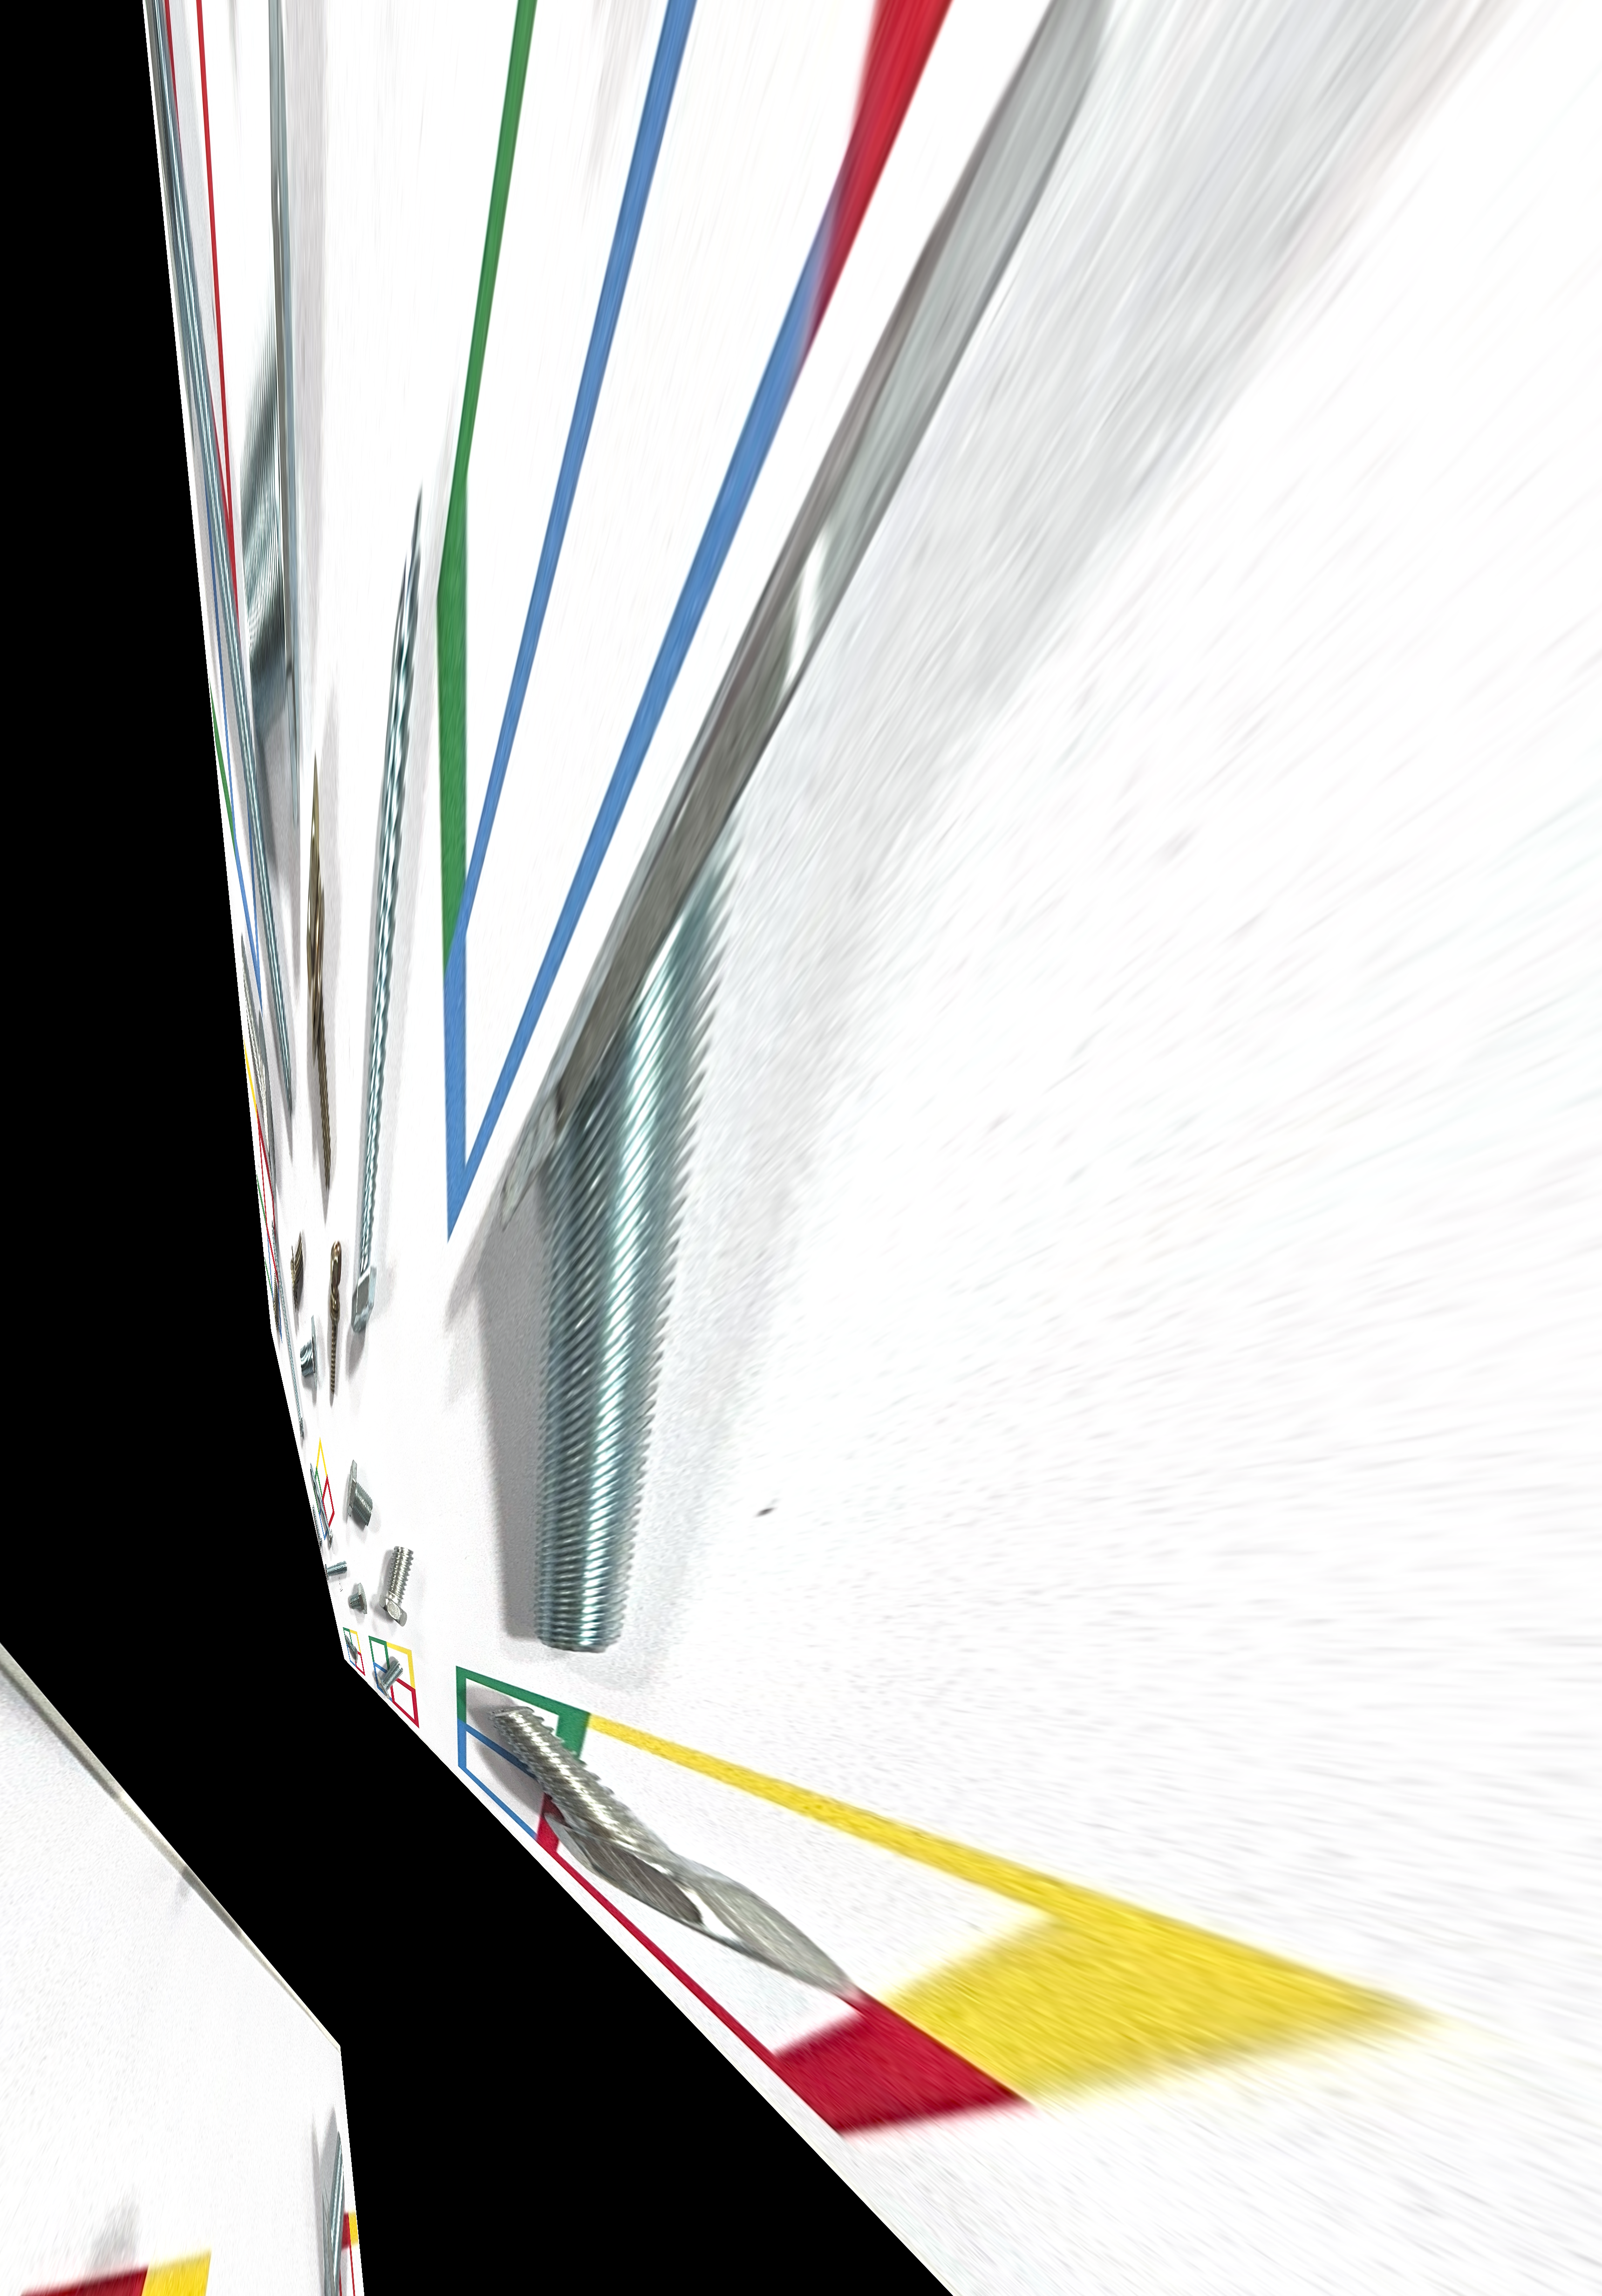
\includegraphics[width=\linewidth]{../523030910004_submission/restored_images/raw_10_warp6.png}
        \caption{原始脚本结果}
    \end{subfigure}
    \hspace{0.01\linewidth}
    \begin{subfigure}[t]{0.26\linewidth}
        \centering
        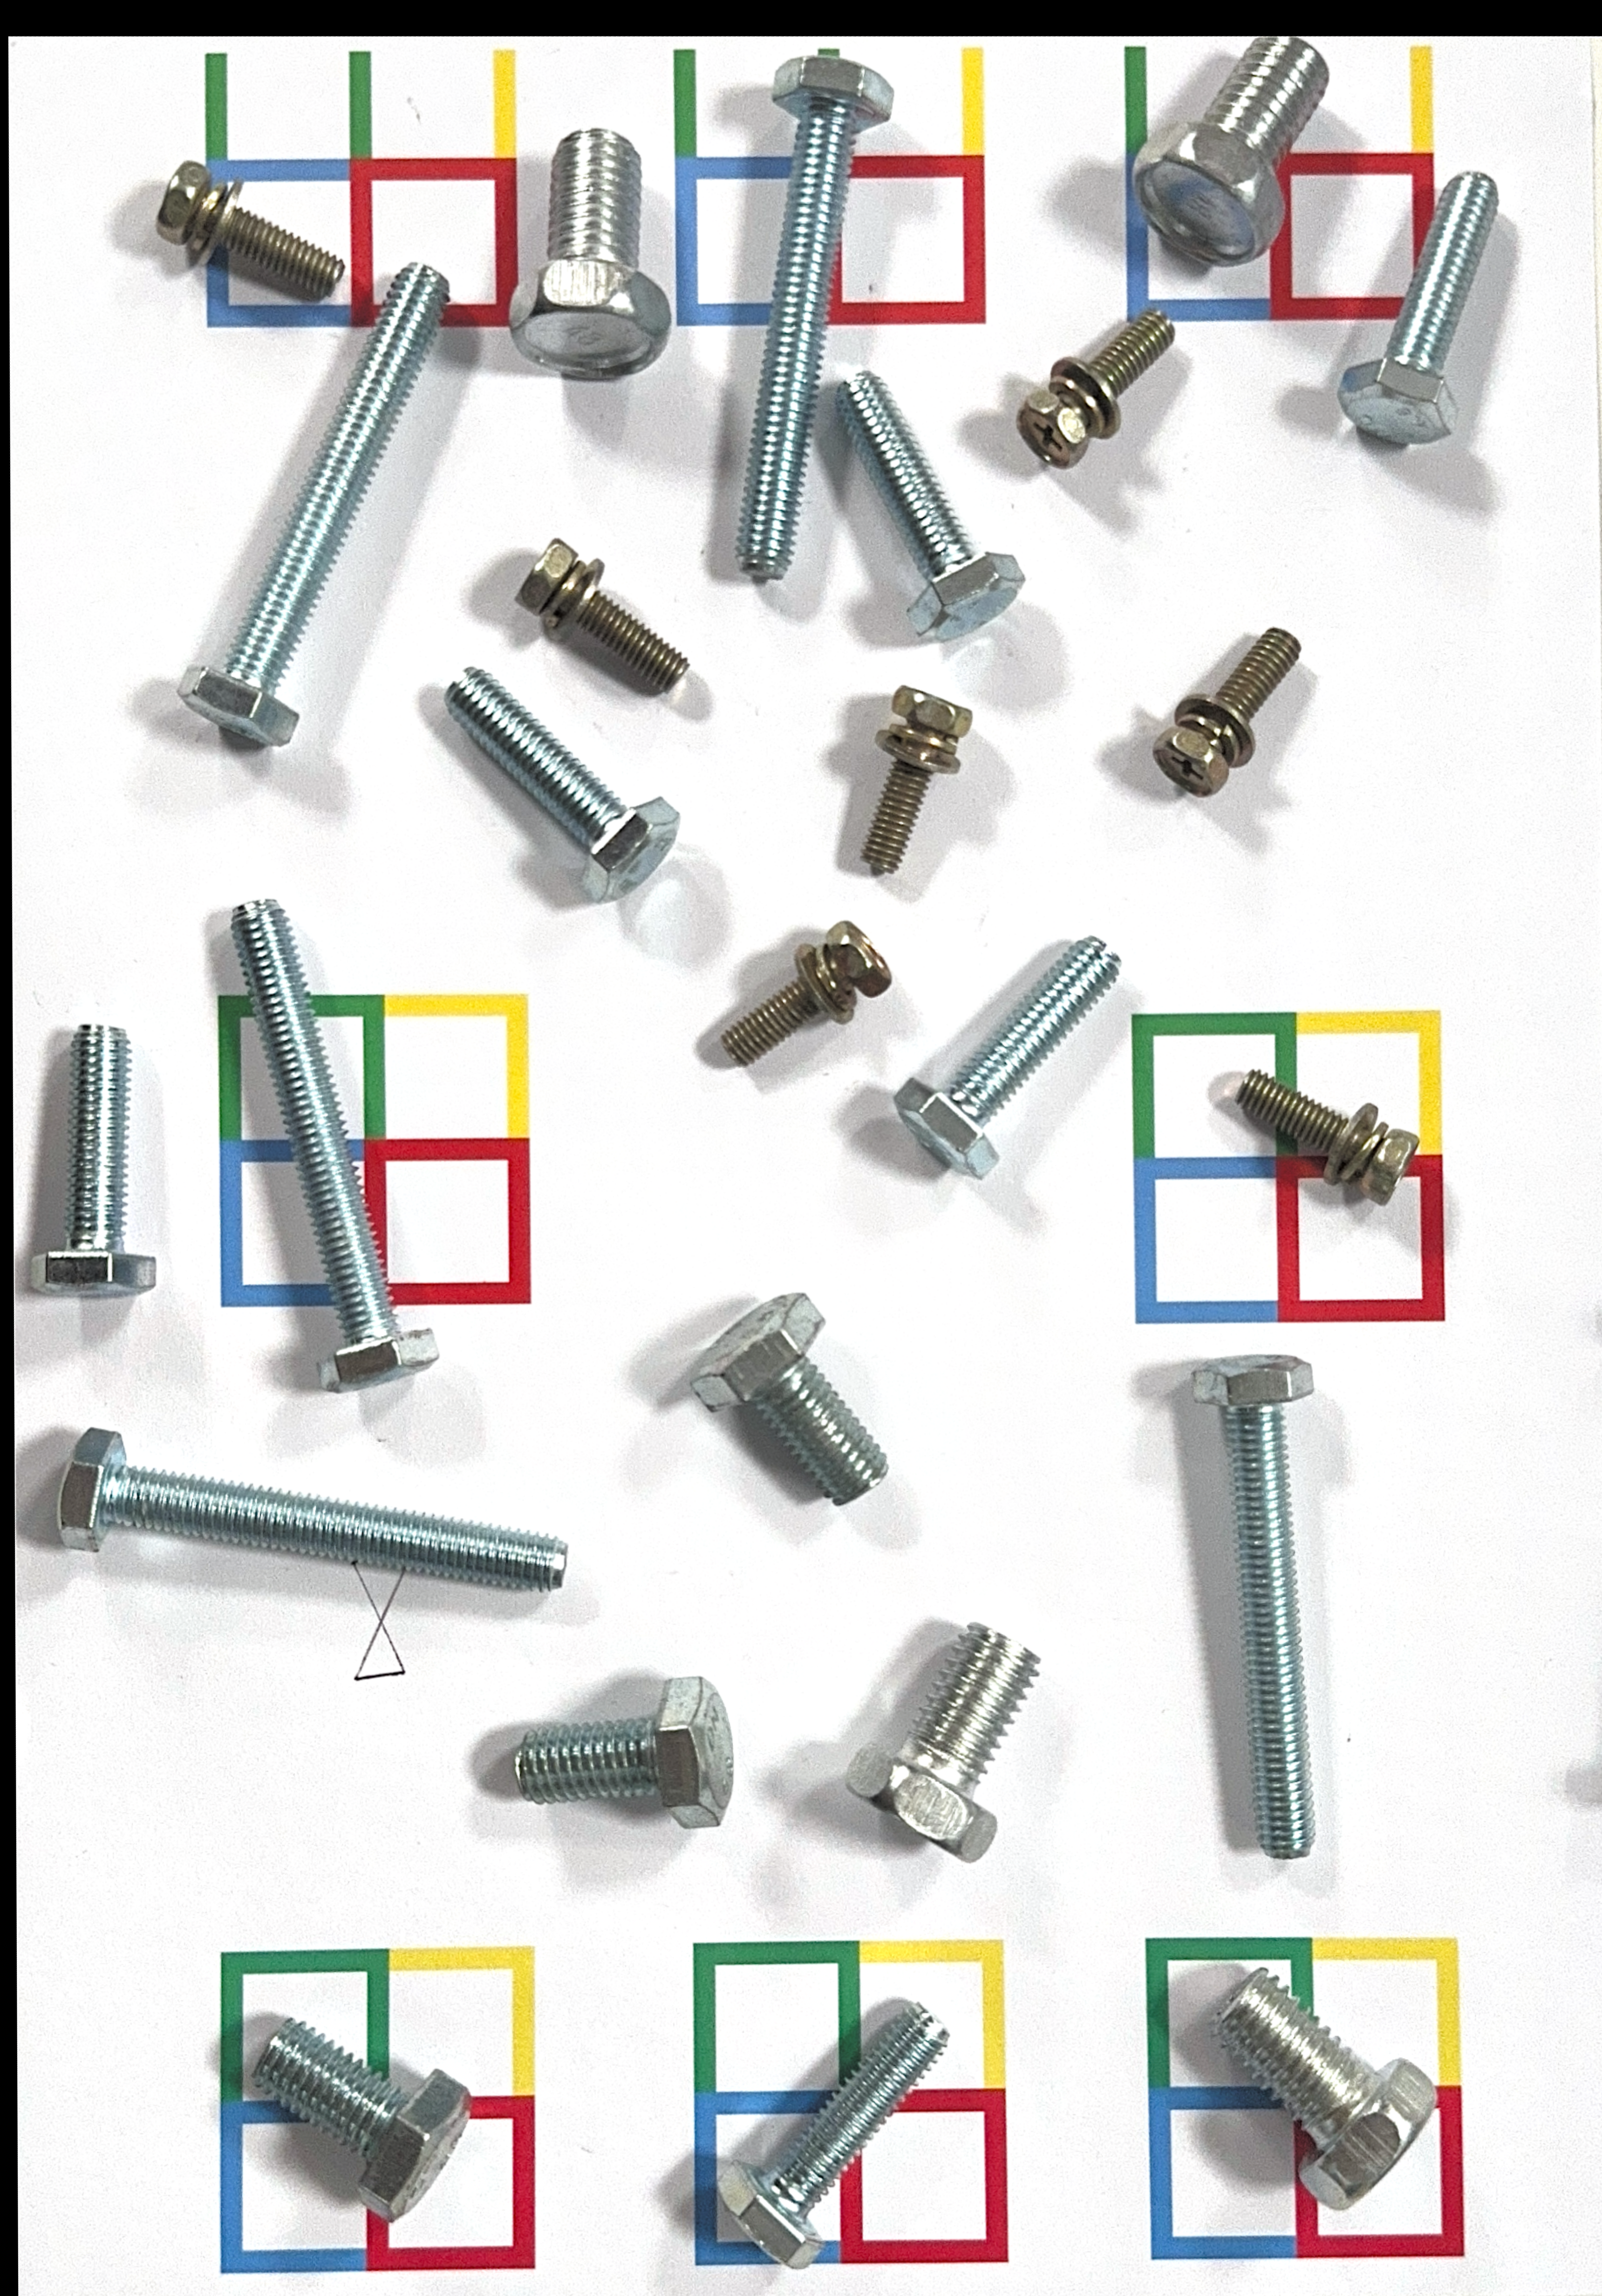
\includegraphics[width=\linewidth]{../523030910004_submission/restored_images/raw_10_warp6_refined.png}
        \caption{改进脚本结果}
    \end{subfigure}
    \caption{raw\_10\_warp6 三图对比}
    \label{fig:refined-compare}
\end{figure}

\section{实验总结与资料}
本次作业完整走通了多视角图像俯视矫正的流程：以模板图为参考，提取关键点与描述子，进行匹配并用 RANSAC 剔除外点，估计单应矩阵后对图像做透视变换，最终输出统一视角的结果图。针对困难样例，还尝试了增加特征点数量、引入 AKAZE 以及均匀采样匹配点等改进，以提升鲁棒性。

通过该实验，我更加理解了单应矩阵如何描述平面之间的几何映射，认识到匹配点分布与误匹配对结果的影响，并体会到鲁棒估计在真实场景中的重要性。同时也学会了根据失败案例定位原因，并通过参数调整与算法组合进行针对性改进。

我查阅了以下资料来进行相关知识的学习：
\begin{itemize}
    \item ORB 特征检测：\url{https://zhuanlan.zhihu.com/p/91479558}
    \item RANSAC 算法：\url{https://zhuanlan.zhihu.com/p/402727549}\newline\url{https://www.cnblogs.com/VisionCoder/p/19325375}
    \item AKAZE 特征检测：\url{https://blog.csdn.net/qq_36812406/article/details/149047702}\newline\url{https://zhuanlan.zhihu.com/p/675066048}
\end{itemize}


\end{document}
